% *********************************************************************
% © 2021 Jeremy Sylvestre
%
% Permission is granted to copy, distribute and/or modify this document
% under the terms of the GNU Free Documentation License, Version 1.3 or
% any later version published by the Free Software Foundation; with no
% Invariant Sections, no Front-Cover Texts, and no Back-Cover Texts. A
% copy of the license is included in the appendix entitled “GNU Free
% Documentation License” that appears in the output document of this
% PreTeXt source code. All trademarks™ are the registered® marks of
% their respective owners.
%
% *********************************************************************

\newcommand*{\xmin}{-6}
\newcommand*{\xmax}{6}
\newcommand*{\ymin}{-2.25}
\newcommand*{\ymax}{2.25}

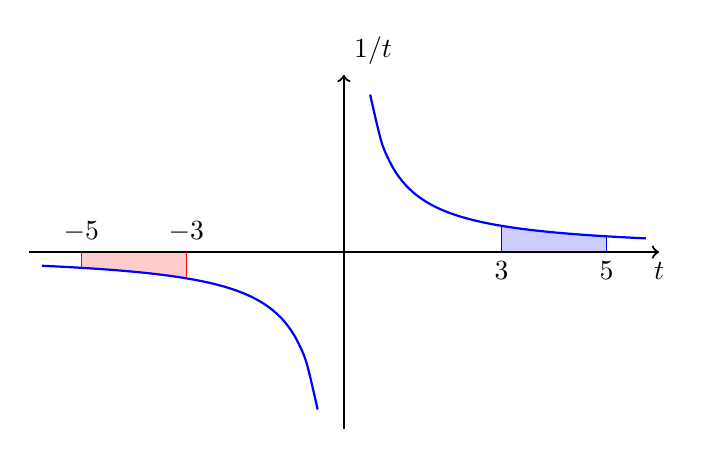
\begin{tikzpicture}
[
	closedpt/.style={circle,draw,fill,inner sep=0pt,minimum size=4pt},
	openpt/.style={circle,draw,inner sep=0pt,minimum size=4pt},
	xscale=0.667
]

	% fills
	\fill[blue, fill opacity=0.2] plot[domain=3:5] (\x,{1 / \x}) -- (5,0) -- (3,0) -- cycle;
	\fill[red, fill opacity=0.2] plot[domain=-5:-3] (\x,{1 / \x}) -- (-3,0) -- (-5,0) -- cycle;

	% axes
	\draw[->,thick] (\xmin,0) -- (\xmax,0) node[below] {$t$};
	\draw[->,thick] (0,\ymin) -- (0,\ymax) node[above right] {$1/t$};

	% graph
	\draw[thick, blue, domain=0.5:5.75, smooth] plot (\x,{1 / \x});
	\draw[blue] (3,0.333) -- (3,0);
	\node[below] at (3,0) {$3$};
	\draw[blue] (5,0.2) -- (5,0);
	\node[below] at (5,0) {$5$};
	% \draw[red] (left) -- (1,0);
	% \node[below] at (1,0) {$1$};
	% \draw[red] (right) -- (0.333,0);
	% \node[below] at (0.333,0) {$t$};

	% graph
	\draw[thick, blue, domain=-5.75:-0.5, smooth] plot (\x,{1 / \x});
	\draw[red] (-3,-0.333) -- (-3,0);
	\node[above] at (-3,0) {$-3$};
	\draw[red] (-5,-0.2) -- (-5,0);
	\node[above] at (-5,0) {$-5$};

\end{tikzpicture}
